%%%%%%%%%%%%%%%%%%%%%%%%%%%%%%%%%%%%%%%%%%%%%%%%%%%%%%%%%%%%%%%%%%%%%%%%%%%%%%%
%% StuPro A, Produktlinien (Kobold)
%% Team Werkbold
%% Angebot
%% $Id: produktanatomie.tex,v 1.1 2004/01/28 18:10:49 garbeam Exp $
%%%%%%%%%%%%%%%%%%%%%%%%%%%%%%%%%%%%%%%%%%%%%%%%%%%%%%%%%%%%%%%%%%%%%%%%%%%%%%%


\chapter{Architekturentscheidungen}

Erg�nzend zum Angebot werden in diesem Dokument die Architekturentscheidungen
n�her erl�utert und ein erweiterter �berblick zum GUI-Prototypen
zusammengefasst, der in der Angebotspr�sentation demonstriert wurde.
\par
\product wird in Form einer {\it J2SE}\footnote{Java 2 Standard Edition,
n�here Informationen unter: http://java.sun.com/j2se/}
 basierten Client-Server Architektur realisiert. Diese Entscheidung
beruht auf der systematischen Abw�gung von Vor- und Nachteilen zwischen
J2SE/Eclipse und GTK/Ada.\par Ada wird von den Werkbold-Entwicklern als
geeignete Entwicklungsumgebung f�r Systeme gesehen, die keine grafische
Benutzungsoberfl�che besitzen sowie f�r einen stand-alone Betrieb
ausgelegt sind, d.h. ohne komplexere Netzwerkanbindung (z.B. Compiler).
Die Anforderungsanalyse ergab hingegen, dass \product als plattformunabh�ngige
GUI-Anwendung mit Netzwerkanbindung realisiert werden soll.\par
Dies spricht in besonderem Ma�e f�r J2SE in Kombination mit der Eclipse
Plattform. Im Folgenden sind die Eigenschaften von J2SE/Eclipse und 
GTK/Ada aufgef�hrt, die zur Entscheidung f"ur die J2SE/Eclipse f"uhrten.\par
Vorteilhaft bewertete Eigenschaften sind mit einem (+) markiert, nachteilig
bewertete Eigenschaften sind mit einem (-) markiert.

\section{Eigenschaften von J2SE/Eclipse}
\begin{itemize}
\item Plattformunabh"angigkeit (+)
\item MVC-Konzept (+)
\item Hoher Verbreitagsgrad (+)
\item Guter Support (Community) (+)
\item Einfache Erweiterbarkeit (+)
\item VCM\footnote{Version Control Management} Unterst"utzung (+)
\item Grafiktoolkit SWT/JFace (+)
\item Gute Dokumentation (IBM) (+)
\item Netzwerktechnologie (+)
\end{itemize}

\section{Eigenschaften von GTK/Ada}
\begin{itemize}
\item Sauberes Sprachdesign (+)
\item Performante Visualisierung (+)
\item Kein natives Widget-Toolkit (-)
\item Abh"angigkeit von GTK (-)
\item "Ubersetzungsvorgang auf"andig (-)
\item Geringer Verbreitungsgrad von GUI-Applikationen (-)
\item Netzwerkanbindung komplex (-)
\item Keine VCM-Unterst"utzung (-)
\end{itemize}

\chapter{Der GUI-Prototyp}

Der Client wird als Plugin f�r die {\it Eclipse Platform}
\footnote{N�here Informationen: http://www.eclipse.org/}
realisiert, das die rollenbasierte Visualisierung und Verwaltung von
Produktlinienarchitekturen in Form von Graphen erm�glicht.\par
Dar�berhinaus dient der Client als Arbeitsumgebung f�r den Produktlinien- und
Produktingenieur sowie f�r den Entwickler. Alle im Produktlinien-Management
notwendigen Workflows k�nnen durch den Client angesto�en und entsprechend visualisiert
werden.

{\begin{center}
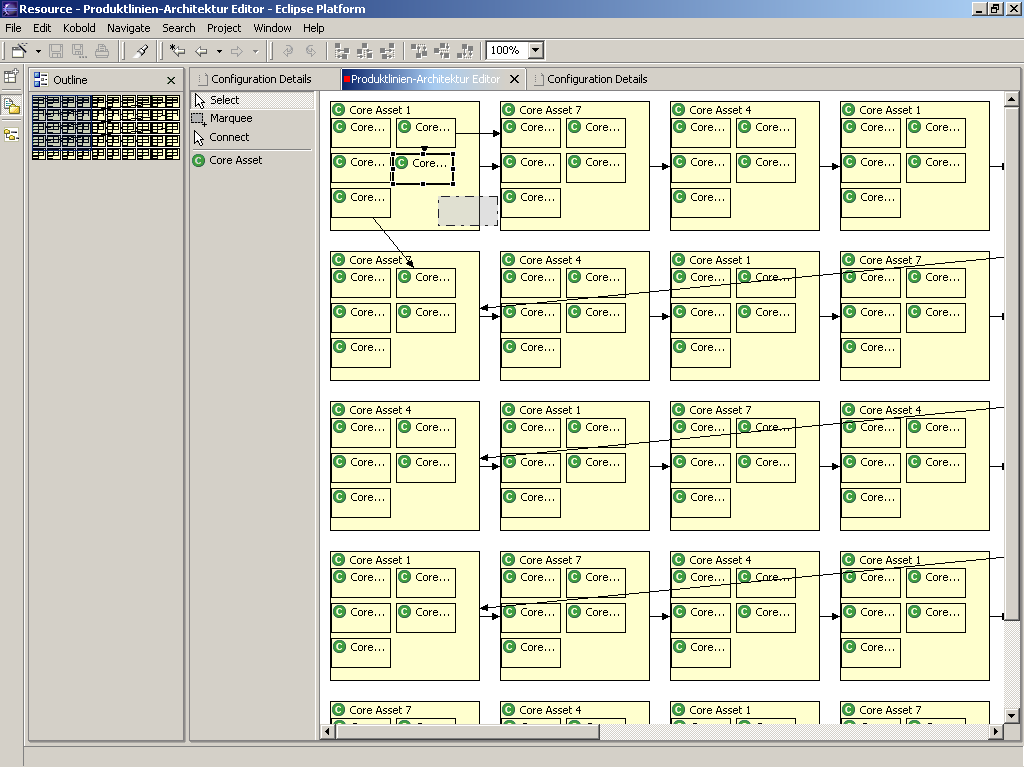
\includegraphics[width=15cm]{kobold-screen}\par
\small Abbildung der Eclipse-basierten Kobold GUI
\end{center}}

\section{Visualisierung}

Der Client visualisiert Produktlinien- und Produkt-Architekturen als Graphen
auf verschiedenen Abstraktionsebenen. Dabei stellt er alle Komponenten und deren
Abh�ngigkeiten (must-use und must-not-use) dar.

{\begin{center}
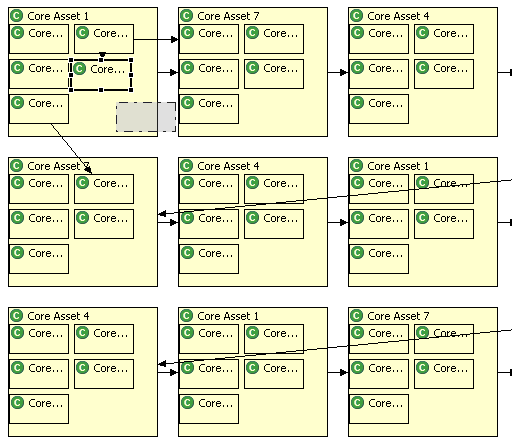
\includegraphics[width=10cm]{visual}\par
\small Ausschnitt aus einem Graphen
\end{center}}

\newpage
\section{Verwaltung}

Der Client verwaltet Produktlinien- und Produkt-Architekturen, d.h. er
erm�glicht die rollenbasierte Erstellung und Modifikation von
Architekturen.

{\begin{center}
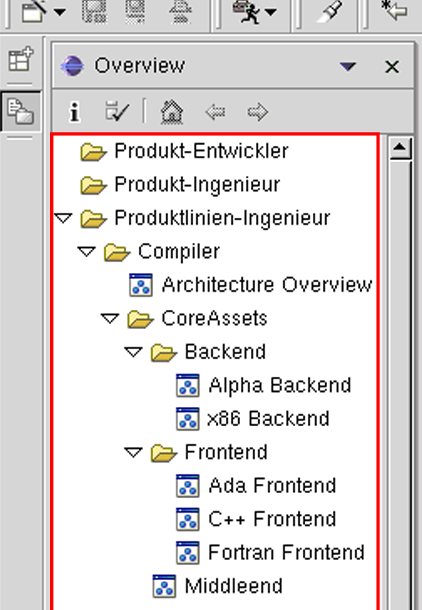
\includegraphics[width=5cm]{verwaltung}\par
\small Ausschnitt der Projektansicht
\end{center}}

\vspace*{2cm}
{\begin{center}
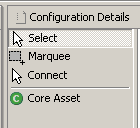
\includegraphics[width=3cm]{verwaltung2}\par
\small Ausschnitt der Manipulationsleiste
\end{center}}

%%% Local Variables: 
%%% TeX-master: "angebot"
%%% End: 
%%% vim:tw=79:
